\documentclass[12pt, letterpaper, titlepage]{article}

\usepackage{amsmath}
\usepackage{amssymb}
\usepackage{booktabs}
\usepackage{amsthm}
\usepackage{graphicx}
\usepackage[margin=1in]{geometry}
\usepackage{hyperref, url}
\hypersetup{colorlinks = true, linkcolor = blue, citecolor=blue, urlcolor =
  blue}
\usepackage{natbib}
\usepackage{enumitem}
\usepackage{setspace}

\usepackage[pagewise]{lineno}
%\linenumbers*[1]
% %% patches to make lineno work better with amsmath
\newcommand*\patchAmsMathEnvironmentForLineno[1]{%
 \expandafter\let\csname old#1\expandafter\endcsname\csname #1\endcsname
 \expandafter\let\csname oldend#1\expandafter\endcsname\csname end#1\endcsname
 \renewenvironment{#1}%
 {\linenomath\csname old#1\endcsname}%
 {\csname oldend#1\endcsname\endlinenomath}}%
\newcommand*\patchBothAmsMathEnvironmentsForLineno[1]{%
 \patchAmsMathEnvironmentForLineno{#1}%
 \patchAmsMathEnvironmentForLineno{#1*}}%

\AtBeginDocument{%
 \patchBothAmsMathEnvironmentsForLineno{equation}%
 \patchBothAmsMathEnvironmentsForLineno{align}%
 \patchBothAmsMathEnvironmentsForLineno{flalign}%
 \patchBothAmsMathEnvironmentsForLineno{alignat}%
 \patchBothAmsMathEnvironmentsForLineno{gather}%
 \patchBothAmsMathEnvironmentsForLineno{multline}%
}

% control floats
\renewcommand\floatpagefraction{.9}
\renewcommand\topfraction{.9}
\renewcommand\bottomfraction{.9}
\renewcommand\textfraction{.1}
\setcounter{totalnumber}{50}
\setcounter{topnumber}{50}
\setcounter{bottomnumber}{50}

\newcommand{\jy}[1]{\textcolor{blue}{JY: #1}}
\newcommand{\eds}[1]{\textcolor{red}{EDS: (#1)}}
\newcommand{\mc}[1]{\textcolor{green}{MC: (#1)}}

\title{On Sample Size for Block Bootstrap Confidence Intervals 
  to Have Desired Coverage Rates}

\author{Mathew Chandy, Elizabeth Schifano,
%   \href{mailto:mathew.chandy@uconn.edu}
% {\nolinkurl{mathew.chandy@uconn.edu}}\\
  and Jun Yan\\[1ex]
  Department of Statistics, University of Connecticut\\
}
\date{}

\begin{document} 
\maketitle

\begin{abstract}
Block bootstrap is widely used in constructing confidence intervals for
parameters estimated from stationary time series. Theoretically, the method
should provide valid confidence intervals as the length of the time series goes
to infinity. In practice, however, it is necessary to know how large of a finite
sample is required for block bootstrap confidence intervals to work well. This
study aims to answer this question in a simple simulation setting where the data
are generated from a first-order autoregressive process. The empirical coverage
rates of several commonly used bootstrap confidence intervals for the mean,
standard deviation, and the lag-1 autocorrelation are compared. In this 
study, we find that a large sample is needed to recover even a simple
parameter like the mean, and that the selection of interval type is very
important, especially in the case of the lag-1 autocorrelation, for which the coverage
deteriorates as the sample size increases when using Percentile, 
%Centered Bootstrap Percentile,
Bias-Corrected, or Bias-Corrected and Accelerated Bootstrap intervals.

\jy{put most
  notable findings here. Possibly 1) large sample is needed; percentile
  bootstrap is not working well for rho (can we offer some explanation?).}

\bigskip
\noindent{\sc Keywords}:
dependent data; resampling; simulation; time series
\end{abstract}

\doublespace

\section{Introduction}
\label{sec:intro}

Block bootstrap is a powerful tool for constructing confidence intervals (CI)
when making inferences about dependent data. Early ideas were developed
independently by \citet{hall1985resampling, carlstein1986use, kunsch1989jackknife}.
It has since been applied in various fields such as econometrics
\citep{mackinnon2006bootstrap} and meteorology \citep{varga2017generalised}.
Block bootstrap is particularly useful for serially dependent
data when the serial dependence is not specified or not of primary interest.
The method is expected to produce CIs with coverage rates
matching their nominal levels as the sample size grows to infinity. However,
when dealing with finite sample sizes, an important question is how large the
sample size needs to be for block bootstrap CIs to have the
desired coverage rates.

The necessary sample size for bootstrap standard errors to provide valid
uncertainty measures in practice has not been extensively studied. For
independent data and non-block bootstrap, \citet{hesterberg2015teachers} notes
that while percentile-based CIs \eds{for the mean? differences in means?} from 
nonparametric bootstrap
are more accurate than $t$-intervals for larger sample sizes, they are
less accurate for smaller sample sizes. \citet{chernick2009revisiting} finds 
that the best choice of method for estimating
the parameter of a distribution is dependent on the sample size, the number of
bootstrap resamples, and the confidence level. In the context of structural equation
modeling, \citet{nevitt2001performance} find
that a sample size of 200--1000 is usually sufficient for interval estimation
using standard nonparametric bootstrap. For dependent data, the necessary
sample
size for bootstrap is even less clear. In the setting of linear regression with a
focus on estimating the proportion of 
variation attributable to a certain variable, \citet{burch2012nonparametric} finds
that three nonparametric bootstrap methods (Standard, Percentile, and Bias-Corrected
and
Accelerated) approach the coverage of a pivotal quantity as $n$ gets larger for an
underlying normal distribution. However, they find that for other distributions, 
coverage may deteriorate as $n$ increases. 
When attempting to create interval estimations for the Pearson correlation 
coefficient of bivariate normal data, \citet{puth2015variety} find bootstrap 
methods to be less accurate than the Fisher's transformation method even 
for a sample of size $n = 100$ and correlation coefficient equivalent to 0.
Few studies have provided a practical guide on what size is needed
for block bootstrap inference for dependent data.
In a linear regression setting
with
dependent data where the
regression errors are generated from a homoscedastic AR(1) process, 
\citet{goncalves2005bootstrap} find that standard error
estimates from moving 
block bootstrap in small samples may be more accurate than
inference from closed-form asymptotic estimates, but moving block bootstrap 
\jy{did they do block or standard bootstrap?}
\mc{moving block bootstrap}
CIs still do not have sufficient coverage of the target parameter even for sample size
$n = 1024$.
\jy{I added more references to the reference folder that studied coverage of
  bootstrap CIs but not block bootstrap CIs.}

The goal of this paper is to provide some practical recommendations on
necessary sample size for block bootstrap with dependent data, similar to what 
was done for basic bootstrap in \citet{hesterberg2015teachers}. We consider a
simple situation of a stationary time series, where the parameters of
interests are the mean, standard deviation, and the first-order
autocorrelation coefficient. We compare six variants of block bootstrap
CIs from the literature \citep{diciccio1996bootstrap,
  rice2006mathematical}: a Standard Normal CI, and a Student's $t$ CI, a Percentile
Interval CI, 
%a Centered Bootstrap Percentile Interval, 
a Bias-Corrected CI, a Bias-Correct and Accelerated($BC_a$) CI, and a CI using a new
Proposed Method. Their
empirical coverage rates at different sample sizes and dependence levels are
compared in a simulation study. The results of this study suggest that
appropriate recovery of temporal dependence parameters is heavily dependent on
the type of interval used.

The remainder of the paper is organized as follows.
Section~\ref{sec:bbci} reviews block bootstrap procedures and how to use block
bootstrap estimates to construct CIs. Section~\ref{sec:simu} reports a
simulation
study comparing the coverage rates of the block bootstrap CIs. A discussion
concludes in Section~\ref{sec:disc}.

\section{Block Bootstrap CIs}
\label{sec:bbci}

Consider a stationary time series $\{X_t: t = 1, \ldots, n\}$ with length~$n$.
Our goal is to construct a CI for a parameter $\theta$ in the
data generating model of the series. Suppose that $\hat\theta_n$ is a point
estimator of~$\theta$ based on the observed series. Bootstrap is a powerful
approach to construct CIs. If the observations in the series
were independent, a standard nonparametric bootstrap procedure would draw a
large number~$B$ bootstrap copies of the observed data, and calculate an
estimate $\hat\theta_n^{(b)}$ for each copy $b = 1, \ldots, B$. The uncertainty
of $\hat\theta_n$ is then estimated by the empirical uncertainty of the
$\hat\theta_n^{(b)}$'s. When serial dependence is present, the bootstrap
procedure needs to preserve the serial dependence. Block bootstrap was
motivated for this situation. 

\subsection{Block Bootstrap}

Block bootstrap preserves the serial dependence in the observed data by
partitioning the data into blocks and performing bootstrap on the blocks.
In particular, consider block size~$l$ and, for convenience, suppose that
$n$ is a multiple of $l$ such that there are $k = n / l$ blocks. Each block~$j$
is $Y_j = \{X_{(j - 1) l + 1}, \ldots, X_{(j - 1) l + l}\}$,
$j = 1, \ldots,   k$.  Then, we sample $k$ blocks of $Y_j$'s from the set 
$\{Y_1, \ldots, Y_k\}$ with replacement and concatenate the $k$ sampled blocks
in the order they are picked to form a bootstrap sample of the data. The
formation of the bootstrap sample ensures that the between-block dependence is
weak and that the within-block serial dependence is preserved. Because the
blocks here are non-overlapping, this bootstrap approach is known as
non-overlapping block bootstrap, or simple block bootstrap.

Alternatively, block-bootstrap can be done with overlapping or moving blocks.
Define moving blocks $Z_j = \{X_j, \ldots, X_{j + l - 1}\}$,
$j = 1, \ldots, n - l + 1$. Now we draw $k$ blocks from the $(n - l + 1)$
blocks
of $Z_j$'s with replacement and then align them in the order they were
picked
to form a block bootstrap sample. If $n$ is not a multiple of~$l$, the last
block selected will be reduced in size so that the final size of the
block bootstrap sample is $n$. It is also possible to implement moving block
bootstrap while allowing blocks to wrap around the end of the series. In other
words, define moving blocks (assuming $l > 1$) as:
\begin{equation}
Z_j =
    \begin{cases}
        \{X_j, \ldots, X_{j + l - 1}\}, & \text{if } j = 1, \dots, n - l + 1,\\
        \{X_j, \ldots, X_n, X_1, \ldots, X_{j-n+l-1}\}, & \text{if } j = n - l
        + 2 ,\dots, n.
    \end{cases}
\end{equation}
This version does not require that $n/l$ be an integer.
We used this version in this study as implemented in the function
\texttt{tsboot} from R package \textsl{boot} \citep{boot}.

The block size~$l$ needs to be chosen with care. It should be large enough for
each bootstrap sample to preserve the serial dependence, yet small enough for
there to be a large number of blocks to give sufficient variability between
each bootstrap sample. As $n$ increases, both~$l$
and $n / l$ should also increase. To achieve this, $l$ is
often assigned a value as a function of $n$. A common function that is
considered optimal is $l = \lceil n^{1/3} \rceil$
\citep{buhlmann1999block}, which was adopted in this study.

\subsection{Bootstrap CIs}

Suppose that we have repeated the steps in the last subsection $B$ times, and
that for $b \in \{1, \ldots, B\}$, we have obtained an estimator
$\hat\theta_n^{(b)}$ based on the $b$th bootstrap sample using the same method
that was applied to $\{X_t: t = 1, \ldots, n\}$ to obtain $\hat\theta_n$.
Now the question is, how to construct a CI for $\theta$
using the $B$ bootstrap point estimates
$\{\hat\theta_n^{(1)}, \ldots, \hat\theta_n^{(B)}\}$.
We consider five kinds of CIs.

\jy{Read carpenter2000bootstrap and cite it; quite useful in sorting the literature}

\paragraph{Standard Normal CI}
Assuming that $\hat\theta_n$ is asymptotically normally distributed with
$\theta$ as the mean, we just need an estimate of the standard error to
construct an approximate CI \citep[p.168]{efron1993introduction}.
Let $\widehat{\text{SE}}$ be the empirical standard error of the block bootstrap
copies of $\hat\theta_n^{(b)}$, $b = 1, \ldots, B$.
A $(1 - \alpha)100\%$ standard normal CI is
\[
(\hat{\theta}_{n} - z_{(1-\alpha/2)}\widehat{\text{SE}}, \quad
\hat{\theta}_{n} - z_{(\alpha/2)}\widehat{\text{SE}}).
\]
\eds{define $z_{(.)}$ and check the signs}
This CI is centered by the point estimator $\hat\theta_n$ and is symmetric.
Its validity relies on whether the distribution of $\hat\theta_n$ is reasonably
well approximated by its asymptotic normal distribution and whether the
bootstrap $\widehat{\text{SE}}$ approximates the true standard error.

\paragraph{Student's $t$ CI}
The procedure for constructing a Student's $t$ CI based on standard bootstrap is
described in \citet{efron1993introduction}. \jy{give page or section number when
  citing a book}
With block bootstrapping, a $(1 - \alpha)100\%$ Student's $t$ CI is
\[
(\hat{\theta}_{n} - t_{(1-\alpha/2), k - 1}\hat{\text{SE}}, \quad
\hat{\theta}_{n} - t_{(\alpha/2), k -1}\hat{\text{SE}}),
\]
\eds{define $t_{(.)}$ and check the signs}
where $k$ is the number of blocks.
This CI is centered by the point estimator $\hat\theta_n$ and is symmetric.
Like the standard 
normal interval, the Student's $t$ CI is a table-based bootstrap interval
approach. In this case,
its validity relies on whether the distribution of $\hat\theta_n$ is
reasonably well approximation by the $t_{k-1}$ distribution with an
expected value of $\theta$, and whether the bootstrap 
$\widehat{\text{SE}}$ approximates the true standard error.

\paragraph{Percentile CI}
The percentile CI was first suggested in \citet{efron1979bootstrap}.
Let $\hat\theta_{n, \alpha}^{(b)}$ be the empirical $100\alpha$th percentile of
$\{\hat\theta_n^{(1)}, \ldots, \hat\theta_n^{(B)}\}$. The $(1 - \alpha)100\%$
empirical percentile CI is
\[
(\hat\theta_{n, \alpha/2}^{(b)}, \quad \hat\theta_{n, 1 - \alpha/2}^{(b)}).
\]
This CI is not necessarily centered by the point estimator $\hat\theta_n$.
As will be shown in our simulation study, this approach works well for the
marginal mean and standard deviation of a serially dependent process, but its
coverage of the temporal dependence deteriorates as $n$ increases, which is
contrary to what one would expect.

%\paragraph{Centered Bootstrap Percentile CI}
%The procedure for constructing a Centered Bootstrap Percentile CI based on
%standard
%bootstrap is
%described in \citet{singh2008bootstrap}.
%The $(1 - \alpha)$ Centered Bootstrap Percentile CI is
%\[
%(2\hat{\theta}_{n} - \hat\theta_{n, 1 - \alpha/2}^{(b)}, \quad
%2\hat{\theta}_{n} - \hat\theta_{n, \alpha/2}^{(b)})).
%\]
%This CI is necessarily centered around the point estimator $\hat\theta_n$ and
%is asymmetric, as different critical values are used to compute
%the lower and upper bounds.

\paragraph{Bias Corrected ($BC$) Bootstrap CI}
The procedure for constructing a Bias Corrected Bootstrap CI based on standard
bootstrap is
described in \citet{carpenter2000bootstrap}.
Let $b = \Phi^{-1}\{\#\{\hat\theta_n^{(b)} < \hat{\theta}_n\} / B\}$
for $b \in \{1, \ldots, B\}$. 
For a $(1 - \alpha)100\%$ CI, let
\[
\alpha_1 = \Phi(2b - z_{\alpha/2}).
\]
\[
\alpha_2 = \Phi(2b - z_{1 - \alpha/2}).
\]
A $(1 - \alpha)100\%~BC$ CI is
\[
(\hat\theta_{n, \alpha_1}^{(b)}, \quad \hat\theta_{n, \alpha_2}^{(b)}).
\]

\paragraph{Bias Corrected and Accelerated ($BC_a$) Bootstrap CI}
The $BC_a$ CI was first suggested in \citet{efron1987better}.
\jy{Isn't this just the empirical CDF? We just need the sample quantile functon.
  What is your reference for this description?}
Let $\hat{z}_0 = \Phi^{-1}\{\#\{\hat\theta_n^{(b)} < \hat{\theta}_n\} / B\}$
for $b \in \{1, \ldots, B\}$. 
Let $Z_{(i)}$ be the original sample without the $i$th block $z_i$, let
$\hat{\theta}_{(i)}$ be the jackknife values of $Z_{(i)}$
for $i \in \{1, \ldots, n\}$, 
and let $\hat{\theta}_{(.)} = \sum_{i=1}^{k} \hat{\theta}_{(i)} / k$. 
Let 
\[
\hat{a} = \frac{\sum_{i=1}^{k} (\hat{\theta}_{(.)} -
  \hat{\theta}_{(i)})^3}{6\{\sum_{i=1}^{k} (\hat{\theta}_{(.)} -
  \hat{\theta}_{(i)})^2\}^{3/2}}
.\] For a $(1 - \alpha)100\%$ CI, let
\[
\alpha_1 = \Phi\left(z_0 + \frac{z_{0} +
  z_{\alpha/2}}{1 - \hat{a}(z_{0} + z_{\alpha/2})}\right).
\]
\[
\alpha_2 = \Phi\left(z_0 + \frac{z_{0} +
  z_{1 - \alpha/2}}{1 - \hat{a}(z_{0} + z_{1 - \alpha/2})}\right).
\]
A $(1 - \alpha)100\%~BC_a$ CI is
\[
(\hat\theta_{n, \alpha_1}^{(b)}, \quad \hat\theta_{n, \alpha_2}^{(b)}).
\]
This CI is not necessarily centered by the point estimator $\hat\theta_n$. The
$BC_a$ method corrects for bias and skewness of the $B$ bootstrap point
estimates $\{\hat\theta_n^{(1)}, \ldots, \hat\theta_n^{(B)}\}$ by including
bias-correction and acceleration factors. The acceleration factor refers to
the 
rate of change of of the standard error of $\hat\theta_n$ with respect to
$\theta$.

\paragraph{Proposed Method CI}
Our Proposed Method CI is centered at the point estimator and uses the
variation
in the bootstrap estimates to construct the error bound. This interval requires
the computation of $\bar\theta_n^{(b)}$, the mean of all bootstrap point
estimates, and $\widehat{\text{bias}} = \bar\theta_n^{(b)} - \hat\theta_n$.
A $(1 - \alpha)100\%$ CI using our Proposed Method is
\[
(\hat\theta_{n, \alpha/2}^{(b)} - \widehat{\text{bias}}, \quad
\hat\theta_{n, 1 - \alpha/2}^{(b)} - \widehat{\text{bias}}).
\]
This CI is necessarily centered around .... and
is asymmetric, as different critical values are used to compute
the lower and upper bounds.

\section{Simulation Study}
\label{sec:simu}

We designed a simulation study to compare the performance of the different
block
bootstrap CI methods. In particular, we generated time series $X_t$
from a 1st order auto-regressive (AR(1)) process:
\[
X_t = \phi X_{t-1} + \epsilon_t,
\]
where $\phi$ is an auto-regressive coefficient, and $\epsilon_t$ is a series of
independent errors from a normal distribution with mean zero and variance
$\sigma_{\epsilon}^2$. The strength of the serial dependence is controlled by
$\phi$, which was set to five levels: $\{-0.4, -0.2, 0.0, 0.2, 0.4\}$.
The series $X_t$ has mean zero and variance
$\sigma_x^2 = (1 - \phi^2) \sigma_{\epsilon}^2$, so for each value of $\phi$,
we
set $\sigma_{\epsilon}^2 = 1 / (1 - \phi^2)$ such that $\sigma_x^2 = 1$.

Three target parameters of $X_t$ were considered:
1) $\mu = 0$, the mean of $X_t$;
2) $\sigma_x = 1$, the standard deviation of $X_t$; and
2) $\phi$, the lag-1 auto-correlation coefficient.
To investigate the effect of sample size~$n$, we considered an array of values
$n \in \{100, 200, 400, 800, 1600, 3200\}$. In each configuration, we generated 
10000 replicates. For each replicate, we constructed seven 95\% block bootstrap
CIs for each parameter as described in the last section. We can estimate 
$\mu$, $\sigma_x$, and $\phi$ by computing the sample mean, sample 
standard deviation,
and lag-1 auto-correlation, respectively, of each bootstrap sample, and then 
construct intervals for each parameter using the appropriate procedures
described in Section~\ref{sec:bbci}.
Then we estimated their actual coverage rates along with their 95\% confidence
intervals from the 10000 replicates. The block bootstrap sampling step was done
with function \texttt{tsboot} from R package \textsl{boot} \citep{boot}, with
block size $\lceil n / l \rceil$. This function by default is an implementation
of moving block bootstrap as described in the previous section, meaning that
that blocks are allowed to wrap around, and $l = \lceil n^{1/3} \rceil$.

\jy{Explain what metric was used to compare their performances. That is, the
  coverage rates and how it was calculated. If a CI is valid, then the coverages
  rate is expected to match its nominal level.}

\jy{Make it flow better and conciser}
The coverage rates of the CIs were used to compare the performance of CIs. Let
$\hat\theta_{L, r}$ and $\hat\theta_{U, r}$ be the lower and upper bound,
respectively, for the confidence interval constructed for each replicate
$r \in \{1, \ldots, R\}$, where $R$ is the
number of replicates.
Then $cov = \#\{\hat\theta_{L, r} < \theta < \hat\theta_{U, r} \}/R$,  
for $r \in \{1, \ldots, R\}$.
If a CI method is valid, then the coverage rate is expected to match the
nominal 
level. Because it is unlikely for the coverage to exactly match the nominal
level,
we can construct a 95\% CI of the coverage
rate (which is an estimate of a proportion with $n = 10000$ \eds{R?}). If the
proportion
0.95 is included in the interval, the block bootstrap method is likely
performing
well. If all values in the interval are below 0.95, the results would suggest 
that the
method either is providing inaccurate estimation, is underestimating the
process' variability, or a combination of both. If all values in the interval
are above .95, the results suggest that the method is overestimating the
process' variability.

If $\theta$ is not covered at that $n$, a larger $n$ may be
necessary, assuming that performance will improve as $n$ is increased.
Remember that
the goal of this study is to find the smallest $n$ which is sufficient for
proper coverage.

The results are graphically displayed in Figures~\ref{fig:mu}--\ref{fig:phi};
these figures were generated using the R \textsl{ggplot2} package
\citep{ggplot2}.

\begin{figure}[tbp]
  \centering
  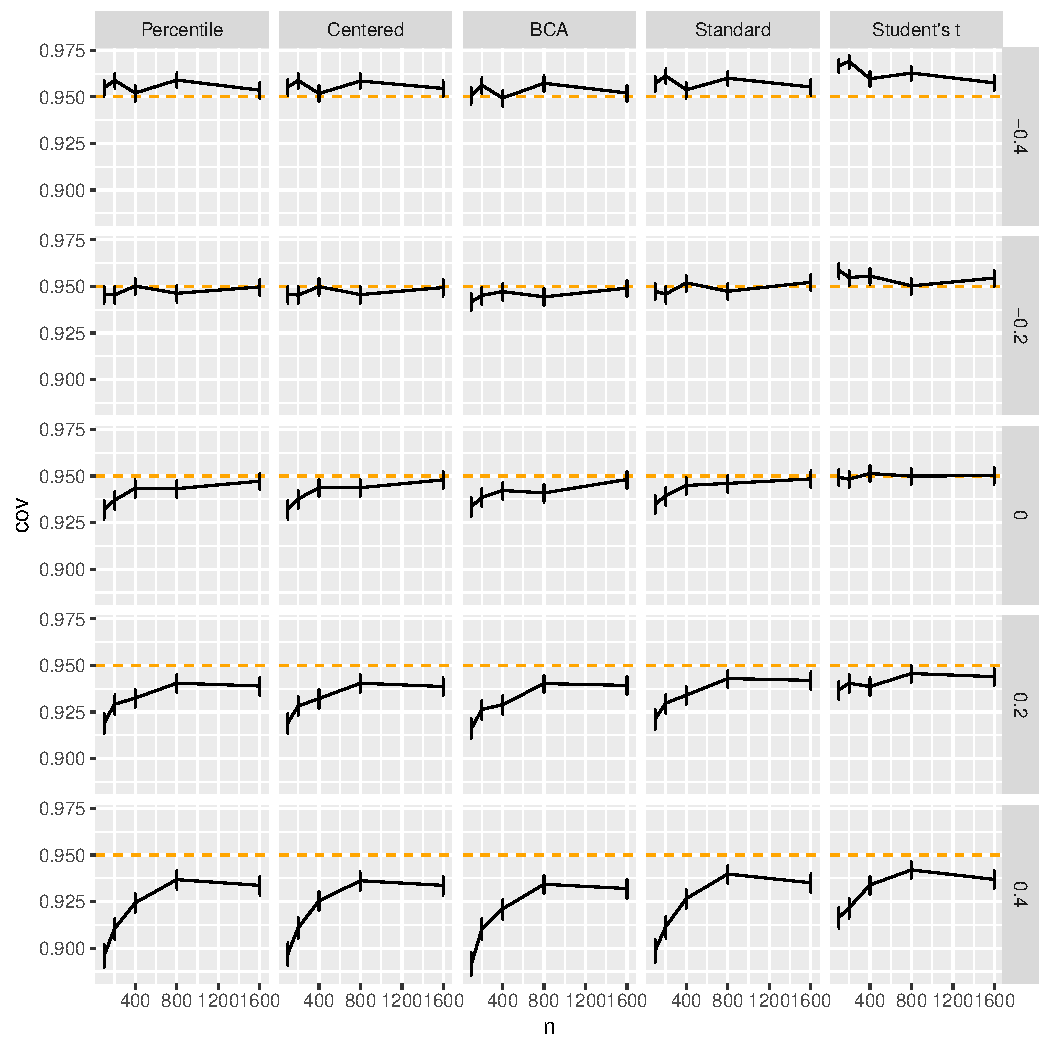
\includegraphics[width=\textwidth]{figures/plot_mu}
  \caption{Empirical coverage rates of different 95\% block bootstrap CIs for
    the marginal mean $\mu$ of an AR(1) process with AR coefficient
    $\phi \in \{-0.4, 0.2, 0, 0.2, 0.4\}$ and series length
    $n \in \{100, 200, 400, 800, 1600, 3200\}$ based on 10,000 replicates.
    The error bars represent 95\% CIs of the real coverage rates.}
  \label{fig:mu}
\end{figure}

\begin{figure}[tbp]
  \centering
  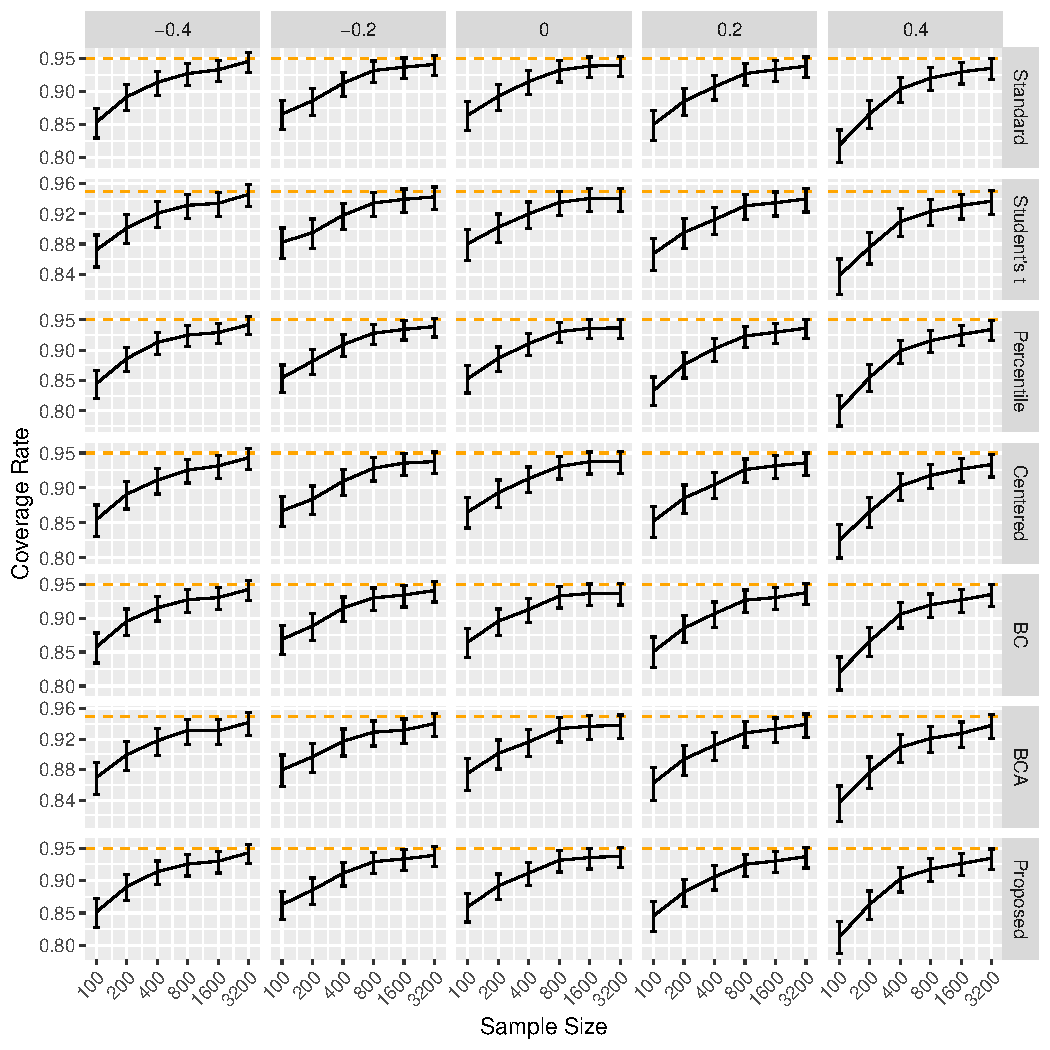
\includegraphics[width=\textwidth]{figures/plot_sigma}
  \caption{Empirical coverage rates of different 95\% block bootstrap CIs for
    the marginal standard deviation $\sigma_x$ of an AR(1) 
		process with AR
    coefficient $\phi \in \{-0.4, 0.2, 0, 0.2, 0.4\}$ and series length
    $n \in \{100, 200, 400, 800, 1600, 3200\}$ based on 10,000 replicates.
    The error bars represent 95\% CIs of the real coverage rates.}
  \label{fig:sigma}
\end{figure}

\begin{figure}[tbp]
  \centering
  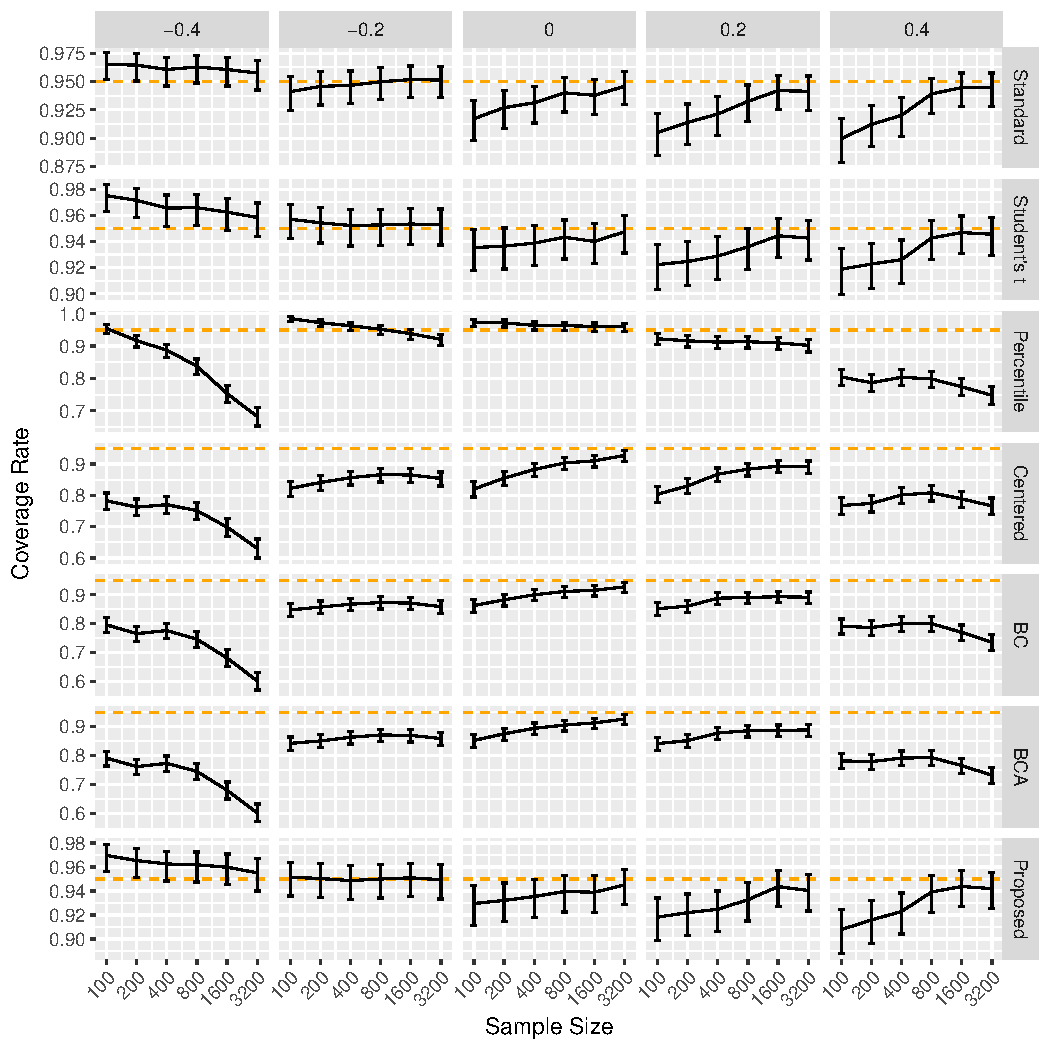
\includegraphics[width=\textwidth]{figures/plot_phi}
  \caption{Empirical coverage rates of different 95\% block bootstrap CIs for
    the first-order autocorrelation coefficient $\phi$ of an AR(1) process with
    $\phi \in \{-0.4, 0.2, 0, 0.2, 0.4\}$ and series length
    $n \in \{100, 200, 400, 800, 1600, 3200\}$ based on 10,000 replicates.
    The error bars represent 95\% CIs of the real coverage rates.}
  \label{fig:phi}
\end{figure}

\jy{I'm curiouss why the coverge is so poor for the percentile method. Could
  plot 50 intervals for phi using different sample sizes?}

Based on Figure~\ref{fig:mu}, 
Student's $t$ CIs appear to have the greatest \eds{largest?} coverage rates with 
respect 
to estimating $\mu$. In fact, for $\phi = -0.4$, Student's $t$ CIs over-cover 
$\mu$ for all sample sizes, whereas other CIs have coverage rates that
hover around the $95\%$ line at this level of $\phi$. For $\phi \geq -0.2$,
$BC_a$ CIs undercover $\mu$ for all $n$ observed. For $\phi = -0.2$, 
Standard, Percentile, %CBP, 
Proposed Method, and $BC$ CIs seem to 
generally cover $\mu$ at the nominal 
rate when $n \geq 400$. Student's $t$ CIs either recover or over-cover $\mu$
for $n \geq 100$. For $\phi = 0$, or when the 
sample is independently normally distributed, $n = 1600$ seems to 
be enough to recover $\mu$ when using Standard, Percentile, 
%CBP, 
Proposed Method, or $BC$ 
CIs. Student's $t$ CIs cover $\mu$ at the nominal rate for $n \geq 100$ at 
$\phi = 0$.
For $\phi = 0.2$, $n > 3200$ seems to be necessary to recover $\mu$
at the nominal level when using
any of the CIs, although some CIs, such as Student's $t$, are much closer to the
$95\%$ line than others, most notably $BC_a$.
For $\phi = 0.4$, a much larger sample size appears to be necessary. Once again,
Student's $t$ CIs are the closest to $95\%$ coverage, and $BC_a$ CIs are the 
furthest.

Based on Figure~\ref{fig:sigma}, 
$BC_a$ CIs greatly undercover $\sigma_x$ for every combination of $n$ and 
$\phi$ observed, although there is no trend of coverage deterioration, 
indicating that there may eventually
be a sample size large enough for $\sigma_x$ to be covered at the nominal level.
For $\phi = -0.4$, Standard Normal and Student's $t$ CIs recover $\sigma_x$ when 
$n = 1600$, but undercover $\sigma_x$ for $n = 3200$, indicating
that a larger $n$ is most likely necessary to consistently cover $\sigma_x$ at 
the nominal rate.
The other CI types undercover $\sigma_x$ for all sample sizes at $\phi = 0.4$.
For $\phi  = -0.2$, all CIs except for $BC_a$ are able to cover $\sigma_x$ at 
the nominal rate for $n \geq 3200$, and Student's $t$ CIs cover $\sigma$ at the 
nominal rate when $n \geq 400$. When $\phi = 0$, $n \geq 1600$ seems to 
be large enough if Standard CIs are used, and $n \geq 400$ is fine is
Student's $t$ CIs are used. $n \geq 3200$ appears necessary 
for other CIs. For $\phi = 0.2$, 
comfortable coverage of $\sigma_x$ at the nominal level appears to only be true
for Student's $t$ CIs for $n \geq 3200$, although Standard %and CBP% 
CIs do reach the nominal level in our simulation results. For $\phi = 0.4$, a much
larger sample size appears to be necessary. Student's $t$ CIs are the closest to
$95\%$ coverage, and $BC_a$ CIs are the furthest.

Based on Figure~\ref{fig:phi}, 
Percentile, %CBP, %
$BC$, and $BC_a$ CIs deteriorate clearly for any level of temporal correlation,
so they should not be used. The deterioration becomes more evident
as the absolute value of $\phi$ increases, regardless of whether $\phi$ is 
negative or positive. When $\phi = -0.4$, Standard and Proposed Method CIs 
recover $\phi$ at the nominal rate for $n \geq 400$. At this $\phi$ level,
Student's $t$ CIs either recover or over-cover $\phi$ for $n \geq 100$. When
$\phi = -0.2$, Standard and Proposed Method CIs recover $\phi$ at $n = 800$ and 
$n = 1600$, 
although they undercover $\phi$ at $n = 3200$, indicating that 
perhaps a larger $n$ is needed if these CIs are used. However,
Student's $t$ CIs cover $\phi$ at the nominal level for $n \geq 400$. When
$\phi = 0$, Standard and Proposed Method CIs recover $\phi$ relatively 
comfortably at $n = 3200$, and 
$n = 800$ seems to be sufficient for Student's $t$ CIs. For $\phi = 0.2$, Standard
and Proposed Method CIs cover $\phi$ at the nominal rate for $n \geq 1600$, whereas 
Student's $t$ CIs can accomplish this at $n \geq 100$. For $\phi = 0.4$, $n \geq 
800$ is large enough for Standard and Proposed Method CIs. Student's $t$ CIs either
recover or over-cover $\phi$ for all $n \geq 100$.

To summarize, the CI type chosen should be based on the target parameter. 
When estimating $\mu$, the Student's $t$ CI seems to have the highest coverage
overall, although that leads to over-coverage when $\phi$ is -0.4. For a
sample with no temporal dependence, the Student's $t$ CI cover $\mu$ perfectly
at the nominal rate even for small sample sizes. For positive $\phi$, a larger
sample size appears to be necessary regardless of the CI used. In the case
that $\phi$ is unknown and expected to be greater than $0$, $n > 3200$ may be
necessary for block bootstrap interval estimation of $\mu$. If $\phi$ is known,
a lesser sample size may be sufficient. When estimating $\sigma_x$,
$BC_a$ should not be used, and Student's $t$ again has the greatest 
\eds{highest?} coverage
rates. In the case that $\phi$ is unknown and expected to be greater than $0$,
$n > 3200$ may be necessary for block bootstrap interval estimation of
$\sigma_x$. Again, if $\phi$ is known, a lesser sample size may be enough.
When estimating $\phi$, Percentile and $BC_a$ CIs 
deteriorate in coverage, indicating they should not be used in this context. 
Increasing $n$ will not fix the performance of either of these intervals 
because the assumption that the coverage rate will approach the nominal level
as $n$ increases is invalid. Standard and Proposed Method CIs managed to fix the
deterioration problem, and they perform similarly, but Student's $t$ covers
$\phi$ at the nominal rate for much smaller sample sizes. It seems that 
$n = 800$ is large enough to
recover $\phi$ when using the Student's $t$ method.

These results beg the question of why certain methods perform poorly. To address 
this question, plots of 100 CIs using each of the Percentile, $BC$, and Proposed 
methods were constructed. 

\begin{figure}[tbp]
  \centering
  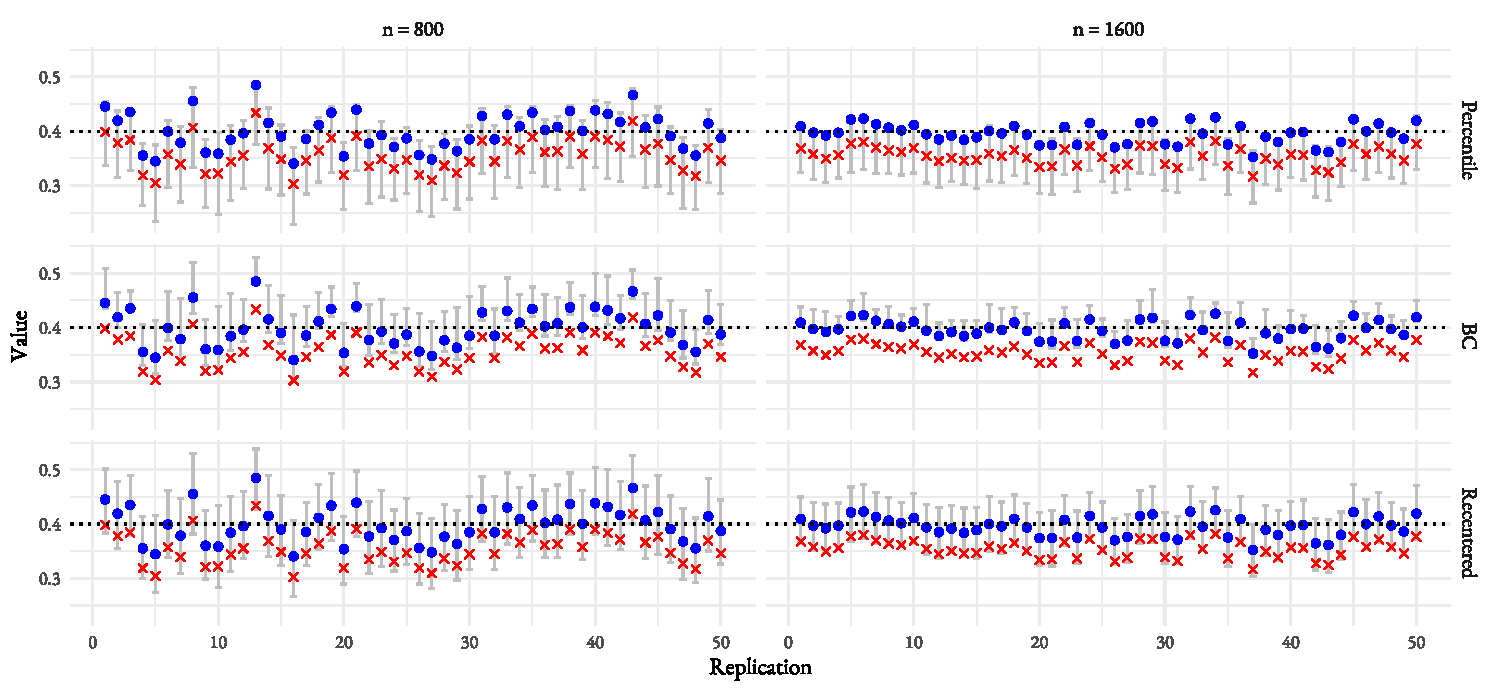
\includegraphics[width=\textwidth]{figures/norm_phi_intervals}
  \caption{100 replicate Percentile, Bias-Corrected, and Proposed Method Bootstrap CIs for samples of $n = 800$ for
    an AR(1) process with $\phi = 0.4$. For each replicate, the lower and upper bounds
    of the CIs are displayed, as well as $\hat\theta_n$ and $\bar\theta_n^{(b)}$. }
  \label{fig:npi}
\end{figure}

As shown in Figure~\ref{fig:npi}, Percentile CIs appear to suffer from bias;
specifically, they seem to heavily underestimate $\phi$. $BC$ CIs do seem to correct this bias on average, but the width of
  the 
CIs is very inconsistent. We can see that the 
Proposed Method CIs correct the bias using 
$\widehat{\text{bias}} = \bar\theta_n^{(b)} -
  \hat\theta_n$, which seems to usually be negative, indicating a positive 
	correction from interval construction in Section~\ref{sec:bbci}.

\section{Discussion}
\label{sec:disc}

\jy{Discussion points:
  1) common practice on block bootstrap even for simple parameter such as the
  mean;
  2) further investigation needed for phi;
  3) impact on applied statsitics courses; student reactions (Dr. Schifano).
}

Block bootstrap is a useful method for estimating parameters of a time
series, from simple parameters like the mean to more complicated temporal
 dependence factors.
%The motivation for the study is the idea that block bootstrap procedure will
%perfectly estimate a parameter of a time series given an infinitely large
%sample. The goal for this study was to find what is a good enough finite
%sample length for block bootstrap estimation to recover the parameter of a
%time series at an acceptable rate.
 We know theoretically that the block bootstrap procedure will cover
  parameter of a time series at the nominal level given an
 infinitely large
sample, so the goal for this study was to find the smallest finite
sample length $n$ of a time series in order for the block bootstrap procedure
to 
recover its associated parameters at an acceptable rate.

Again, this analysis relies on the assumption that
there is a size $n$ large enough for the method to work: that is, the method's
performance improves as $n$ increases. Out of the five types of intervals used
in this study, this assumption was found to hold true with respect to
estimating $\phi$ only for Standard, Student's $t$, and Proposed Method CIs, 
whereas Percentile, 
%CBP, 
$BC$, and $BC_a$ intervals exhibited coverage deterioration as $n$
increased. The Percentile CI's coverage deterioration can be attributed to
bias that is not corrected as $n$ increases. Specifically, as $n$ increases, 
the width of the CI decreases, but because the Percentile CI
underestimates $\phi$, the coverage decreases. The $BC$ CI seems to correct the 
bias, but the width of the CI seems to be inconsistent. The acceleration 
factor of the $BC_a$ CI seems to fail, as the width of the CI
seems to be inconsistent. 

When using Student's $t$ intervals and $\phi$ is
unknown, the results of this study suggest that an $n > 3200$ may be
necessary for common practice to estimate simpler parameters like $\mu$ 
or $\sigma_x$. If $\phi$ is already known, a lesser $n$ may be adequate
to
estimate these parameters. For lower absolute values of $\phi$, a smaller
$n$ is sufficient when estimating $\mu$ or $\sigma$. For negative
values of $\phi$, coverage of $\mu$ is higher in general. In fact, 
Student's $t$ seems to over-cover $\mu$ for $\phi = 0.4$, 
meaning that if $\phi$ is known to have a very negative value, another CI
should be used.
However, in real world applications, $\phi$ is
more commonly found to be positive, so Student's $t$ should still be used
if $\phi$ is unknown.
Lastly, to estimate $\phi$, an $n$ of around $800$ using the 
Student's $t$ method
 may be sufficient.
Further investigation may be necessary to see if there are other interval
corrections that fix the coverage deterioration problem for $\phi$.

This study could be used as a guide for applied statistics courses for students
to generally understand how large of a sample size is sufficient for block
bootstrap to be used versus other inference methods.
This information could also prove to be useful for research using block
bootstrap
estimation of time series in domains such as econometrics. Future studies
could investigate if there are types of block bootstrap interval
construction such as $ABC$ or bootstrap-t intervals
that would more appropriately recover the parameters of a time
series. \eds{are there other methods that you know of?} 
One could also investigate the $n$ needed to make inferences about
other forms of serially dependent data such as a moving average process. 

\bibliographystyle{chicago}
\bibliography{citations}

\end{document}
